\documentclass{article}
\usepackage[utf8]{inputenc}

\title{Graph Kernels and Support Vector Machines for Pattern Recognition}
\author{\textbf{Léo Andéol}\thanks{leo.andeol@gmail.com}\\ Master DAC, Sorbonne Université\\ Paris, France}
\date{May 2019}

\usepackage[square,sort,comma,numbers]{natbib}
\usepackage{graphicx}
\usepackage{amsmath,amsthm,amssymb}
\usepackage{mathtools}
\usepackage{multicol}
\usepackage{url}
\usepackage{todonotes}
\usepackage{lipsum}

\DeclarePairedDelimiter{\abs}{\lvert}{\rvert}
\DeclarePairedDelimiter{\norm}{\lVert}{\rVert}

\let\vec\mathbf
\newcommand*{\C}{%
  \mathbb{C}%
}
\newcommand*{\R}{%
  \mathbb{R}%
}
\newcommand*{\Z}{%
  \mathbb{Z}%
}

\newtheorem{theorem}{Theorem}
\theoremstyle{definition}
\newtheorem{definition}{Definition}

\begin{document}

\maketitle
\begin{abstract}
	The problem of having a framework to classify graphs is becoming increasingly important in the era of data. The issue has been tackled since the beginning of the millennium and there have been significant progress. This report introduces all necessary knowledge to understand the topic and then reviews different graph kernels while focusing on a random walk kernel and its optimization. Some experiments are then conducted to verify the information given by the state of the art, and some attempts are made to accelerate the different methods to compute the kernel.  
\end{abstract}

\newpage

\tableofcontents

\newpage

\section{Introduction}
 \todo{introduction générale plus étendue : 1 et 1/2 page :donner un aperçu/résumé du rapport : un paragraphe par élément - ECRIRE A LA FIN}
 \paragraph{}Nowadays the world is turning to a new era where data is the most valuable resource, and we are working on algorithms to exploit those the best way possible. Most research is currently focused on the so-called "big data", huge quantities of data which are very sparse and of poor quality. However, there also exist structured databases of good quality, in the form of graphs, which is the one we will be studying. Graphs can be very useful in various fields, but is partly known for its use in biology, as it can be used to represent proteins or other types of molecules.
 \paragraph{}Classification of such graphs is an important problem of pattern recognition which affects a lot of sectors such as medicine, biology, and more. It was studied since the start of the millennium and significant progress was made : several methods were discovered and gave good results but met a big issue, the complexity of those methods. Since then, the main objective of research on this topic has been to either find more computationally efficient algorithms, or to find methods to accelerate the ones already in use.
 \paragraph{}The first part of this report will introduce all the necessary background knowledge that is graphs as already mentioned, but also Support Vector Machines (SVMs) which is the classification algorithm we will be using and kernels which are transformations of data usually used to increase the accuracy of SVMs. However, graphs being non-vector data, kernels have also the objective of becoming a metric of comparison between two instances of graphs. Thus, the main principles of graph kernels will be introduced as well as their definitions. Afterwards, the different methods used to improve the computation complexity of the kernel will be introduced together with their own complexities, advantages and disadvantages.

\paragraph{}The second part of this report will be focused on the technical side and experiments conducted during the project. A synthetic graph database made of toy data was required to conduct simple and quick experiments on to verify the claims made in the main publication studied, in different cases such as labeled and unlabeled graphs, or varying the size of either the database of the graph studied. Different challenges and problems met during the implementation will be explained, as well as their solution, if one has been found. Then, the main subject of this part will be discussed : the accuracy and computation time of different methods, estimation of their complexities and different attempts to approximate those methods. Finally, an experiment on a real database of proteins\todo{voir si j'en fait plus} is conducted, and the results analyzed.
 
\section{Methodology}
\subsection{Background}
sous section 1 : background : graphe, svm, noyaux, donner toutes les définitions.
\subsubsection{Graphs}
\todo{Revoir toutes les refs}
A graph\cite{graph_wiki} is a type of mathematical structure that represents connections between objects. It is thus composed of vertices (or nodes) and edges. Vertices represent objects and are usually depicted as circles or spheres whereas edges link pairs or vertices. 
\begin{definition}
	A graph is an ordered pair $G=(V,E)$ where :
	\begin{itemize}
		\item $V$ is a set of nodes
		\item $E \subseteq \{(u,v) : (u,v) \in V^2\}$
	\end{itemize}
\end{definition}
\begin{figure}[!htb]
\begin{multicols}{2}
    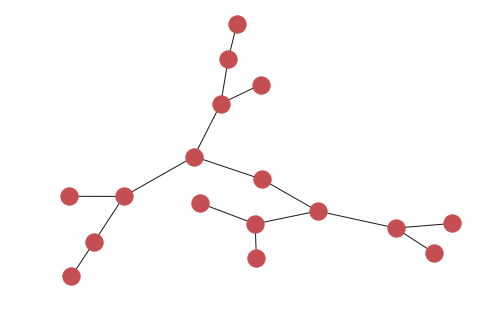
\includegraphics[width=\linewidth]{data/graphs/big_graph_no_label.png}\par
    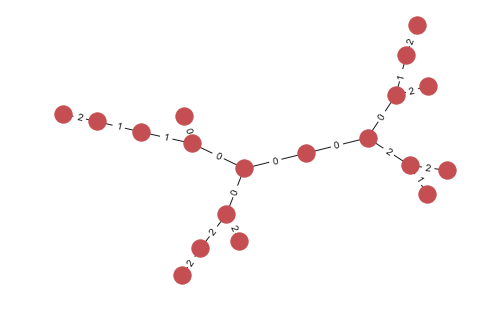
\includegraphics[width=\linewidth]{data/graphs/big_graph_label.png}\par
\end{multicols}
\caption{Two "tree" graphs, resp. unlabeled and labeled}
\end{figure}
The edges of the graph can be weighted and can be either oriented or not. We will be focusing on undirected unweighted graphs.
\begin{definition}
	Let $G=(V,E)$ be a graph, if $G$ is undirected, then we have
	\begin{itemize}
		\item $\forall (u,v) \in E \implies (v,u)\in E$
	\end{itemize}
\end{definition}
\paragraph{Degree}
\begin{definition}
	The degree of a vertex $d(v)$ is the number of vertices it is connected to.
\end{definition}
It is ... ?
\begin{definition}
	A path
\end{definition}
\begin{definition}
	A cycle
\end{definition}
\paragraph{Labels and colors}
Both vertices and edges can have labels (sometimes called colors), they can take various forms : they can be integers, elements of a finite or infinite set (such as integers but also strings), or even continuous (such as $\in \R$).
\paragraph{Connectivity}
Connectivity is another basic concept of graphs. It means that all vertices are accessible from any vertex.
\begin{definition}
	Let $G=(V,E)$ be a graph,\\
	$G$ is connected if and only if there is a path between every pair of vertices
\end{definition} 
If a graph is a not connected, and a subgraph induced by it is, then this subgraph is called a connected component.
\\
Graphs were first used in their modern form to represent the problem of Seven Bridges of Königsberg (cite), and have been ever since used to represent maps, and thus path-finding algorithms were developed. Graphs can also be used, with labels, to represent different type of molecules and interactions between them.(parler aussi des réseaux ? des problemes de flots etc ?)\\
During this project, we will focus on undirected graphs which can have any type of labels on their edges only (if it is only on their nodes, the complementary graph can be studied).\\
We will be comparing graphs in order to find similarities between them, and classify them in different groups. It has been shown(cite) that it can be used effectively on proteins and (?).
\subsubsection{Support Vector Machines}
Support Vector Machines (SVM) are a type of machine learning algorithms discovered in the early 90s(cite). It was originally a classification algorithm however it has been expanded since to regression and clustering too. It is especially powerful and widely used for two main reasons :
\paragraph{Margin and support vectors}
The Support Vector Machines were based on the model of the Perceptron (cite), another classification algorithm that tried to find an hyperplane that discriminates the two sets.\\
The main issue with the Perceptron is that it had no formal guarantee to find an optimal hyperplane, and more often than not would not find it. Moreover, if the data weren't linearly separable, the algorithm would not converge.\\
In order to tackle theses issues, the SVM offered three fixes. \\
First, they added a margin in the loss function in order to not only classify well the data samples, but also with the maximum certainty, i.e. as far from the decision boundary as possible.\\
\begin{equation}
    L(y,x,w) = \max(0,-y*x \cdot w) \implies L(y,x,w) = \max(0,1-y*x\cdot w)
\end{equation}
Then, seeing this solution wasn't enough, as there was still an infinity of possible solutions, it was proven that the margin between points and the decision boundary was inversely proportional to the norm of the weights.\\
\begin{equation}
\gamma = \frac{y_{i}(x_{i} \cdot w + w_{0})}{\norm{w}}
\end{equation}
These two fixes gave us the first version the SVM, the hard-margin SVM :\\ 
\begin{equation}
    \min \frac{1}{2}\norm{w}^{2} \quad
\textup{s.t.}\quad y_{i}(x_{i} \cdot w + w_{0}) \geq 1 \quad \forall i \in \{1..n\}
\end{equation}
However, if the data weren't linearly separable the algorithm wouldn't be optimizable since the quadratic programming problem requires all points to be correctly classified. Then, a new term $\xi$ was introduced as an error tolerance, as well as a factor $C$ that would determine the balance between error tolerance and weights minimization.\\
\begin{equation}
\begin{array}{ll@{}ll}
\text{min}  & \frac{1}{2}\norm{w}^{2}+C\sum\limits_{i=1}^{n}\xi_{i} &\\
\text{s.t.}& \forall i \in \{1..n\} & y_{i}(x_{i} \cdot w + w_{0}) \geq 1-\xi_{i}
\end{array}
\end{equation}
\subsubsection{Kernels}
In its dual form, the SVM problem only requires a dot product between the sample vectors. Then, we can use a nonlinear transformation $\phi(x)$ to replace the dot-product $\vec{x_i} \cdot \vec{x_j}$ by $\phi(\vec{x_{i}})\cdot\phi(\vec{x}_{j})$ , effectively augmenting the dimensions of our vectors and thus the expressiveness of our model by enhancing the separability of the data. However, for complex transformations, such as in infinite dimensions, the function $\phi$ isn't defined. But it was found(cite) that the standard dot product can be replaced by another function as long as it is a bilinear positive semi definite form. 
\begin{definition}
	A kernel $K$ is positive semi definite if and only if :\\
    \begin{equation}
    	\sum\limits_{i=1}^{n}\sum\limits_{i=1}^{n}K(\vec{x_{i}},\vec{x_{j}})c_{i}c_{j} \geq 0 \qquad \forall i \in \{1..n\} \quad c_i \in \R
    \end{equation}
\end{definition}
Thus, the dot product can be replaced by a function $K(x_1,x_2)$ which will indirectly (?) transform the data in larger dimensions, even infinite with the Gaussian kernel(cite) and return the dot product of those transformations, while remaining computable in all cases. This replacement is usually called the "Kernel Trick".\\
Ever since the foundation of SVMs, the kernel trick became a big focus of the machine learning community as it naturally fits in the algorithm and allows supervised learning on very complex data, and enjoying greater accuracy than most algorithms.
\subsection{State of the Art}
\todo{Mettre explication comme "ici nousallons parler de ça ça " ou pas}
\subsubsection{Introduction}
In this chapter we will discuss the advance of research on graph kernels.Graph Kernels are a type of R-convolution kernels\cite{haussler99convolution} applied to graphs, which are kernels that are based on decompositions of complex objects and comparisons of those decompositions.\\
Graph Kernels have been studied since Support Vector Machines started getting popular\cite{kashima_graphkers_2003}. Since then, a lot of progress has been made, and several types of kernels have been discovered\todo{découverts ou inventés?}, such as random walk\cite{kashima_graphkers_2003} and graphlet\cite{shervashidze_efficient_2009} kernels, the two we will be studying, but not the only ones. There are also graph kernels that use spanning trees, and several others that are unfortunately usually not positive semi-definite\cite{shervashidze_scalable_2012}.
\subsubsection{Graphlets}\todo{A faire plus tard}
A graphlet\cite{shervashidze_efficient_2009}\todo{Citer deux fois un seul article ok ou pas?} is a subgraph of 3,4 or 5 nodes taken from a much larger graph. The idea of a graphlet kernel is to count all types of graphlets that appear in a graph, and use that count to compare to another graph.\\
insert list of graphlets
\subsubsection{Random walks}
Graph kernels based on Random Walks have been studied since very early\cite{kashima_graphkers_2003}, several of them were created and were then united\cite{vishwanathan_graph_2010}. Random walks are a type of rather intuitive algorithms : the idea is to randomly walk through a graph and then compare it to random walks in another graph. Actually, all the random walks are computed at the same time by making the adjacency matrix stochastic and using it as a Markov chain. Moreover, it has also been shown\cite{imrich_prodgraphs} that performing a walk on two separate graphs at the same time is the same as performing a walk on the product graph. The product graph is in simpler terms the Cartesian product of the two graphs, taking all possible combinations of nodes and linking those nodes when there is an edge between two specific nodes in both the original graphs. \\
\begin{definition}
	Let $G_1=(V_{1},E_{1})$ and $G_2=(V_{2},E_{2})$ be two graphs,\\the product graph
	$G_\times = (V_{\times},E_{\times})$ is then defined as
	\begin{itemize}
		\item $V_{\times} = \{(v,w) : v \in V_{1}, w \in V_{2} \}$
		\item $E_{\times} = \{((v_1,w_1),(v_2,w_2)) : v_1,v_2 \in V_{1}^2, w_1,w_2 \in V_{2}^2 \}$
	\end{itemize}
\end{definition}
However, technically, the adjacency matrix $W_{\times}$ of a such graph is the result of the Kronecker (tensor) product of the two adjacency matrices $A$ and $A_2$ of the two graphs \cite{imrich_prodgraphs,noauthor_kronecker_2019}:
\begin{equation}
    W_{\times}=A \otimes A_{2}
\end{equation}
We will also need the $vec$ operator that is very linked to the tensor product :
\begin{definition}
	Let $A$ be a matrix $n\times n$, $vec(A)$ is the vector obtained by stacking all columns of $A$.
\end{definition}

\subsubsection{Kernel definition}
\todo{finir}
The kernel is defined as follows
\begin{definition}Let $p_{\times}$ and $q_{\times}$ be respectfully the start and end probability of each node, and let $W_{\times}$ be the adjacency matrix of the product graph of $G$ and $G'$, and finally $\mu(k)$ be a convergent function of $k$.
	\begin{equation}
		k(G,G') = \sum\limits_{k=0}^{\infty}\mu(k)q_{\times}^{\top}W_{\times}^{k}p_{\times}
	\end{equation}
\end{definition}

\subsubsection{Sylvester Equation}
A Sylvester equation, also sometimes called Lyapunov equation (we will stick to Sylvester here) is a matrix equation of the following shape :
\begin{definition}
	Let $A$, $B$, and $C$ be matrices of compatible shapes, then the Sylvester equation is
	\begin{equation}
	AX+XB=C
	\end{equation}
	And the discrete-time Sylvester Equation is 
	\begin{equation}
	AXB+C=X
	\end{equation}
	Which can be generalized as
	\begin{equation}
		\sum_{i=0}^{d}A_{i}XB_{i}=X
	\end{equation}
\end{definition}
We will be exclusively using the discrete-time Sylvester Equation and its generalization and will be referring to it as Sylvester equation. These equations are solved usually using Schur decompositions in $O(n^3)$ for the basic Sylvester equation and in unknown time for the generalized version\cite{vishwanathan_graph_2010}.\\
We can use this equation to solve our kernel faster by replacing the $A$ and $B$ matrices by our adjacency matrices $A_1$ and $A_2$, adding $\lambda$, and $C$ by our start probabilities $p_\times$ while vectorizing the whole equation thus obtaining :\todo{colon or not?}
\begin{equation}
	vec(M) = vec(\lambda A_{1}MA_{2}) + p_{\times}
\end{equation}
From which we can obtain (where I is the identity matrix)\todo{partie speciale pour notations?}
\begin{equation}
	q_{\times}^{\top}vec(M)=q_{\times}^{\top}(I-\lambda W_{\times})^{-1}p_{\times}
\end{equation}
Thus, having calculated the inverse kernel by an alternative method. The advantage of this method is that it is very fast, but unfortunately limited to unlabeled graphs, unless there is an implementation for the generalized Sylvester equation. Moreover, compared to the others, this option is very simple and does not require specific parameters, but like many others, suffers when it encounters singular matrices. 
\todo{donner des exemples = comme quoi}

sous section 2 : state of the art : graph kernels et acceleration des random walk, donner les complexité, donner des exemples, discuter avantages et inconvenients chacun
\subsubsection{Conjugate Gradient Method}
The Conjugate Gradient Method is an optimization algorithm used to find approximate solutions of linear systems that have a positive semi definite matrix. As its name suggests, it is a gradient based (usually) iterative algorithm. The Main idea is  
assumes as geometric $\mu(k)$ function
\subsubsection{Fixed Point Iterations}
\todo{Faire usage de fct paragraph ??}
A fixed point is a value for which a function, returns that same value :
\begin{definition}
	Let $S$ a set and $f$ a map $f : S \implies S$,\\
	$x \in S$ is a fixed point of $f$ if and only if $x=f(x)$ 
\end{definition}
Fixed point iterations is a method of computing a fixed point of a function by applying repeatedly the following equation until $\norm{x_{n+1}-x_{n}}<\epsilon$ where $\epsilon$ is the acceptable level of error.
\begin{equation}
	x_{n+1} = f(x_n)
\end{equation}
There is also a guarantee of convergence :
\begin{theorem}
	In order for the fixed-point iterations to converge, it is necessary that $\lambda<|\xi|^{-1}$ where $\xi$ is the largest eigenvalue of $W_\times$
\end{theorem}
\todo{le mettre en appendix?}
\begin{proof}
  Let $x_0=p_\times$ and $t>>0$
  \begin{align*}
      x_{t+1}-x_t &= p_\times+\lambda W_{\times} x_t - x_t &\\
      &= p_{\times}+(\lambda W_{\times} - 1)(p_{\times}+\lambda W_{\times} x_{t-1})\\
      &= p_{\times} - p_{\times} + \lambda W_{\times}p_{\times} + (\lambda W_{\times})^2 x_{t-1} - \lambda W_{\times} x_{t-1}\\
      &= \lambda W_{\times}(p_{\times}-x_{t-1}+\lambda W_{\times} x_{t-1}) \\
      &= \lambda W_{\times}(p_{\times}-\lambda W_{\times} x_{t-2} - p_{\times} + \lambda W_{\times}(\lambda W_{\times} x_{t-2} +p_{\times}) \\
      &= \lambda W_{\times} ( \lambda W_{\times} (\lambda W_{\times} x_{t-2}+p_{\times}-x_{t-2})) \\
      &= (\lambda W_{\times})^2(\lambda W_{\times} x_{t-2}+p_{\times} - x_{t-2}) & \\
      \text{We find a pattern}\\
      \implies x_{t+1}-x_t &= (\lambda W_{\times})^t (\lambda W_{\times} x_0 + p_{\times} - x_0) & \\
      \text{And because } x_0 = p_{\times}\\
      &= (\lambda W_{\times})^{t+1} p_{\times}\\
      \text{Which decreases only when}\\
      \xi_1 < 1\\
      \text{The largest magnitude eigenvalue of} \lambda W_{\times}\\
      \implies \lambda < |\xi_1|^{-1}
      && \qedhere
  \end{align*}
\end{proof}
Since this method requires the computation of $W_\times$, the kernel value can be computed for any type of labeling. For unlabeled graphs, the complexity is $O(kn^3)$ and $O(kdn^3)$ for labeled graphs, where $d$ is the number of labels and $k$ the number of iterations which can be estimated by:
\begin{equation}
	k=O\left(\frac{\ln \epsilon}{\ln \lambda + \ln \abs{\xi}}\right)
\end{equation}
Finally, the fixed point iterations is more demanding than the others since it has a condition on the value of $\lambda$ and thus assumes as geometric $\mu(k)$ function, and the number of iterations can easily vary a lot\todo{verifier sur graphes}. The only advantage of this method is that it is very simple while still being better than the raw kernel.
\subsubsection{Spectral Decomposition}

\subsubsection{Nearest Kronecker Product Approximation}
\url{https://mathematica.stackexchange.com/questions/91651/nearest-kronecker-product}
\url{http://citeseerx.ist.psu.edu/viewdoc/download?doi=10.1.1.42.1924&rep=rep1&type=pdf}\cite{VanLoan1993}
\subsection{Contributions}
en anglais ça donne ?



\section{Experiments}
\todo{experiences : détailler db, tests, méthodes, les parametres, construction label, donner tableaux, resultats, teps de calculs, précision, discuter tout cela}
A big part of this project consisted in implementing the different algorithms from the main paper that I had studied \cite{vishwanathan_graph_2010}, verifying the results obtained in that article, and making new attempts to accelerate those algorithms while keeping the best accuracy possible.
\subsection{Implementation}
Implementing code from the main paper was a challenge in itself. Several problems aren't really documented and finding functions to solve them, or even explanations on how to solve them is sometimes difficult.
\subsubsection{Graphs}
The first thing that had to be done was to create a graph database generator, of very simple and standard graphs that had expectable behaviors and could thus be used for tests. Those graphs would also be altered using simple transformations, in order to create different graphs belonging to the same class.\\
\begin{figure}[!htb]
	\begin{multicols}{4}
		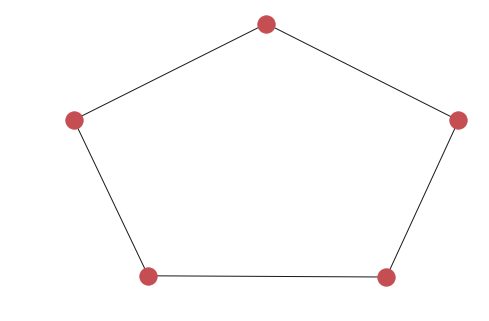
\includegraphics[width=\linewidth]{data/generated-graphs/ring_base.png}\par
		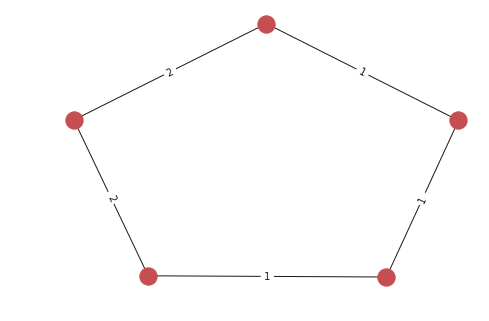
\includegraphics[width=\linewidth]{data/generated-graphs/ring_labels.png}\par
		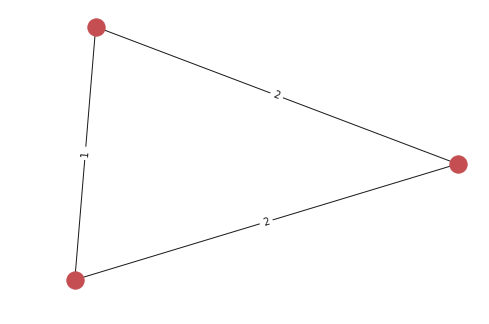
\includegraphics[width=\linewidth]{data/generated-graphs/ring_altered_struct.png}\par
		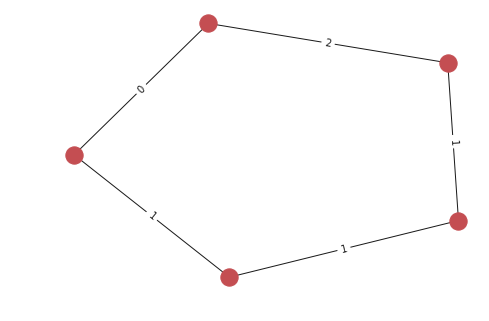
\includegraphics[width=\linewidth]{data/generated-graphs/ring_altered_labels.png}\par
	\end{multicols}
	\caption{Ring graphs, resp. unlabelled, labelled, altered structured, altered labels}
\end{figure}
For simplicity, it was decided to only use 3 classes to stay as simple as possible. We studied 3 standard types of graphs : the ring, the star and the tree. A ring graph is a connected graph where each vertex is connected to exactly two vertices, it thus forms one big cycle. A star graph is composed of a central node, and of several other nodes that are all and only connected to the central node, it should look like a star, or perhaps a flower.\todo{Est-ce que je devrais dire ça ?}. Finally, a tree is a famous type of graph : it is a connected graph without any cycles, but here we will be studying a special type of tree, since each vertex is at most of degree 3.\\
\begin{figure}[!htb]
	\begin{multicols}{4}
		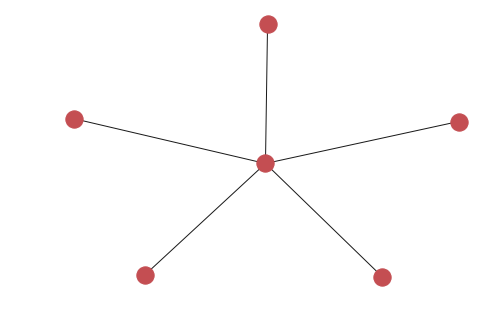
\includegraphics[width=\linewidth]{data/generated-graphs/star_base.png}\par
		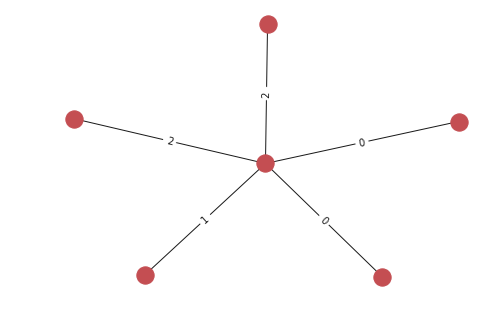
\includegraphics[width=\linewidth]{data/generated-graphs/star_labels.png}\par
		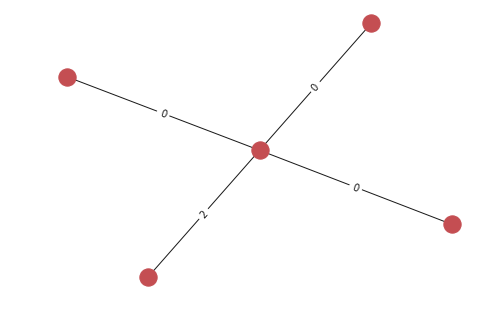
\includegraphics[width=\linewidth]{data/generated-graphs/star_altered_struct.png}\par
		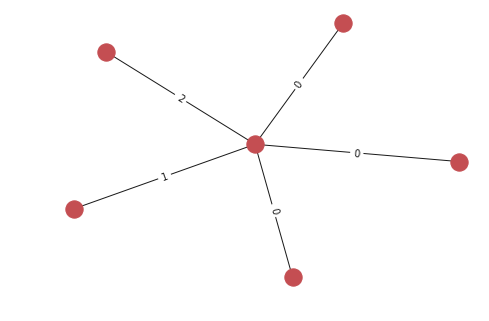
\includegraphics[width=\linewidth]{data/generated-graphs/star_altered_labels.png}\par
	\end{multicols}
	\caption{Star graphs, resp. unlabelled, labelled, altered structured, altered labels}
\end{figure}
The database generator works as follows:\todo{verifier si anglais, et c'est ok mettre deux points ?} for each type of graph, it will create a graph of predetermined size with randomly generated edge labels in a certain given interval. Then, for each graph, it will alter it a predefined number of times, and each time will create a new graph that has been both altered on structure and on labels. Alteration on structure involves removing or adding a predefined number of nodes in respect of the type of the graph thus staying in the same class as the source. 
\begin{enumerate}
	\item Ring graphs are simply regenerated slightly longer or shorter randomly.
	\item Star graphs are also regenerated either with more or less nodes, randomly.
	\item Tree graphs are either expanded by adding randomly leaves anywhere in the graph, or reduced by randomly removing leaves.
\end{enumerate}
Alteration on labels will randomly switch a predefined\todo{predefined beaucoup répété, c'est un probleme ?} number of edge labels. Once this is done, the generator will create two databases out of the set of previously generated graphs, one will be made of the adjacency matrix of each graph without looking at labels, and the second one will be an array of adjacency matrices taken from graphs induced by selecting only edges with a specific label, and that for all labels in the label set.
\begin{figure}[!htb]
	\begin{multicols}{4}
		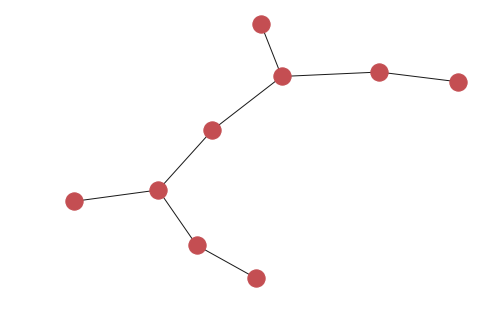
\includegraphics[width=\linewidth]{data/generated-graphs/tree_base.png}\par
		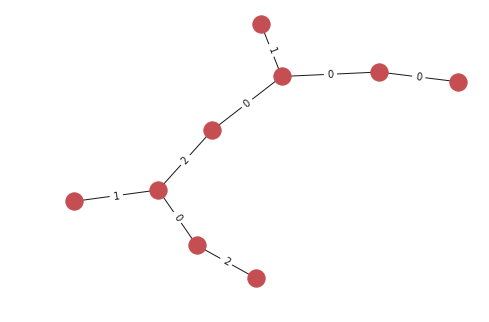
\includegraphics[width=\linewidth]{data/generated-graphs/tree_labels.png}\par
		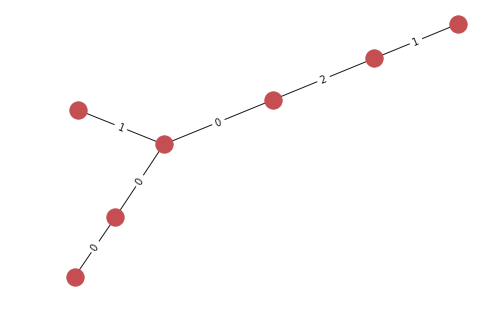
\includegraphics[width=\linewidth]{data/generated-graphs/tree_altered_struct.png}\par
		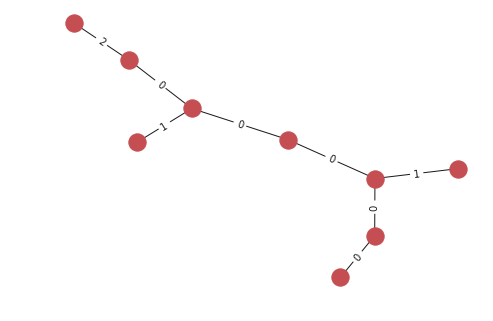
\includegraphics[width=\linewidth]{data/generated-graphs/tree_altered_labels.png}\par
	\end{multicols}
	\caption{Tree graphs, resp. unlabelled, labelled, altered structured, altered labels}
\end{figure}
\subsubsection{Raw Kernel}
\subsubsection{Inverse Kernel}
\subsubsection{Sylvester Equation}
The Sylvester Equation is a good example of poorly documented problems (compared to the others). There are very few resources on the subject, and even less implementation of solvers. We could theoretically use the Sylvester Equation on both labeled and discrete-labeled graphs which are respectfully represented as Sylvester and Generalized Sylvester Equations (involving a sum of matrices), however, the only library available solves the first one, but not the second one. There seems to be confusing terminology\todo{correct ?} since there is a solver for the Generalized Sylvester Equation, but a different one than the one described in our source\cite{vishwanathan_graph_2010}. The same source also mentions a way to solve the generalized version\cite{lathauwer2004}, however, this option wasn't explored.  
\todo{changé ça ?}
\todo{Rajouter papier à citer}
\subsubsection{Conjugate Gradient Method}
Note : Preconditioner random vector : $x \cdot x^{T}$ fonctionne bien\\
The Conjugate Gradient Method is however very well documented\cite{nesterov_lectures_2018} and there are several libraries implementing this algorithm (we will be using scipy).
\todo{a faire}
\subsubsection{Fixed Point Iterations}
Rapidité de la convergence : géométrique avec un ratio $\lambda$1/$\lambda$2???
si lambda trop proche de l'inverse de la valeur propre peut etre tres lent à converger quand la matrice d'adjacence est très dense\\
The Fixed Point Iterations method was very easy to implement and gave rapidly good results, however there is a constraint on the lambda(the geometric factor) used in the kernel as we have proved. Experiments showed that a lambda very close to the constraint increases significantly the time of computation to convergence.\todo{image}

\subsubsection{Spectral Decompostion}
can't inverse Left eigenvectors : 
\url{https://arxiv.org/pdf/1708.00064.pdf}
\subsubsection{Nearest Kronecker Product}
\url{https://www.sciencedirect.com/science/article/pii/S0377042700003939?via%3Dihub}
	\url{https://www.imageclef.org/system/files/CLEF2016_Kronecker_Decomposition.pdf}
	\url{http://dx.doi.org/10.1007/978-94-015-8196-7_17}
	\url{https://mathematica.stackexchange.com/questions/91651/nearest-kronecker-product}
	

\subsection{Test of the random walk kernel}
\subsubsection{Accuracy comparison between labelled and unlabelled graphs}
Même score, car donne même matrice ???
\begin{table}[!htb]
\begin{center}
\begin{tabular}{|l|l|l|}
    \hline
    & Unlabelled & Labelled \\
    \hline
    Accuracy & ? & ? \\
    \hline
    Time & ? & ? \\
    \hline
\end{tabular}
\end{center}
\caption {Time and Accuracy of learning resp. for unlabelled and labelled graphs} \label{tab:lab_vs_nolab} 
\end{table}

\subsubsection{Efficiency of alternate methods}
\begin{table}[!htb]
\begin{center}
\begin{tabular}{|p{15mm}|p{15mm}|p{15mm}|p{15mm}|p{15mm}|p{15mm}|p{15mm}|p{15mm}|}
    \hline
    & Raw\newline kernel & Inverse\newline Kernel & Sylvester\newline Equation & Conjugate\newline Gradients & Fixed\newline points & Spectral\newline Decomp. & Nearest\newline Kronecker Product \\
    \hline
    Accuracy & 67\% & 67\% & ? & 67\% & 67\% & ? & ? \\
    \hline
    Time & 18.40s  & 5.72 & ? & 7.62s & 5.94s & ? & ? \\
    \hline
\end{tabular}
\end{center}
\caption {Time and Accuracy of learning for the raw kernel and other methods} \label{tab:kernel_comparison} 
\end{table}
\subsubsection{Experiments on a biology dataset}
\url{https://ls11-www.cs.tu-dortmund.de/staff/morris/graphkerneldatasets} 
\url{http://members.cbio.mines-paristech.fr/~nshervashidze/code/}
enzymes

\subsection{Comparison of kernels}
\subsubsection{Label use}
Comparison using labels and no labels
\subsubsection{Comparison of their gram matrices}
The algorithms approximate the kernel using very different techniques, thus the gram matrices obtained from the kernels were similar in appearance, but had significant differences of scale. It was then decided to normalize very simply the gram matrices so they could be more easily compared.
\begin{equation}
	M = (M - min(M) )/max(M)
\end{equation}
\begin{figure}[!htb]
	\begin{multicols}{2}
		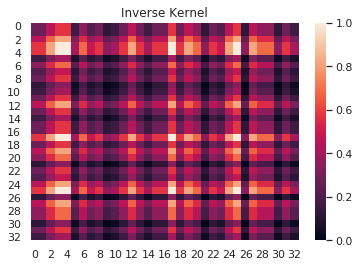
\includegraphics[width=\linewidth]{data/gram/gram.png}\par
		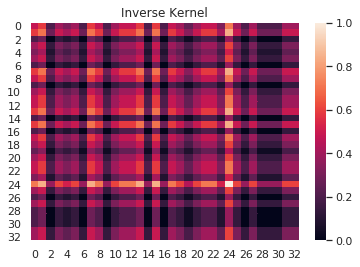
\includegraphics[width=\linewidth]{data/gram/gram2.png}\par
	\end{multicols}
	\caption{Two gram matrices computed using the Inverse Kernel on different datasets}
\end{figure}
Afterwards, in order to verify all the algorithms gave similar results, it was decided to compute the Frobenius norm of the difference of two gram matrices (divided by the size of the matrix, thus giving the mean standard deviation). The following results were obtained and were satisfying.
\begin{table}[!htb]
\begin{center}
\begin{tabular}{|p{15mm}|p{15mm}|p{15mm}|p{15mm}|p{15mm}|p{15mm}|p{15mm}|p{15mm}|}
	\hline
	& Raw\newline kernel & Inverse\newline Kernel & Sylvester\newline Equation & Conjugate\newline Gradients & Fixed\newline points & Spectral\newline Decomp. \\
	\hline
	Raw. & 0 & 1.1e-4 & 9.8e-5 & 8.9e-5 & 1.0e-4 & 1.0e-04  \\
	\hline
	Inv. & - & 0 & 2.1e-5 & 7.9e-5 & 4.0e-6 & 6.8e-6 \\
	\hline
	Syl. & - & - & 0 & 8.0e-5 & 1.7e-5 & 1.4e-5  \\
	\hline
	Con. & - & - & - & 0 & 7.9e-5 & 7.9e-5  \\
	\hline
	Fix. & - & - & - & - & 0 & 2.8e-6 \\
	\hline
	Spe. & - & - & - & - & - & 0 \\
	\hline
\end{tabular}
\end{center}
\caption {Approximate standard deviation of matrix entries (?)}
\label{tab:frobenius_norm_diff} 
\end{table}
\todo{correct nom ?}
Indeed, the 

\subsubsection{Complexity and Accuracy}

\subsubsection{title}

\subsection{Individual kernel analysis ?}
\todo{mettre ici les images variations degré d'approximation}
\subsection{Nearest Kronecker product ?}

\subsection{On molecules}

\subsection{Improvements}

\section{Conclusion and Future Work}
experiences : détailler db, tests, méthodes, les parametres, construction label, donner tableaux, resultats, teps de calculs, précision, discuter tout cela
section 4 : 1 page ou page et demi : conclusion et discussion


\appendix
\section{Appendix}
\section{Annex 1}

\section{Acknowledgements}
This work was done during the first year of my master.

\listoffigures
\listoftables
bibliographie et index

\bibliographystyle{ieeetr}
\bibliography{references}
\end{document}
